\chapter{Proposta de Solução} \label{chap:proposta}

% Este capítulo apresenta a abordagem proposta para o descarregamento de tarefas em redes de Computação de Borda Veicular (\gls{VEC}). A solução consiste em um agente de Aprendizado por Reforço Profundo (\gls{DRL}) baseado no algoritmo \gls{PPO}, cujo espaço de observação é estruturado de forma invariante à escala por meio do método multicritério \gls{FUZZY-TOPSIS}.

Este capítulo apresenta uma proposta de solução para o problema de descarregamento de tarefas em ambientes veiculares, contemplando a comunicação tanto com dispositivos de borda quanto diretamente entre os dispositivos instalados nos veículos. Um desafio central abordado nesta modelagem é a não estacionariedade, um fenômeno intrínseco aos sistemas multiagente resultante da interação e da coadaptação contínua entre os diversos agentes \cite{albrecht2024}. Para garantir que a simulação espelhe com precisão as restrições do mundo físico, o modelo incorpora comportamentos complexos e variáveis de incerteza, tais como a mobilidade dinâmica veicular, cargas de trabalho baseadas em traços reais de uso, limitações de processamento (\textit{throttling}) e atrasos na propagação de informações \cite{albrecht2024}. Consequentemente, a introdução desses elementos estabelece um ambiente de simulação rigoroso e estocástico, projetado para imitar as limitações operacionais e os ruídos de comunicação enfrentados em cenários reais \cite{albrecht2024}.

\section{Ambiente}

\begin{figure}[htb]
    \centering
    \resizebox{\textwidth}{!}{%
    \begin{tikzpicture}[
        font=\sffamily,
        >=Stealth,
        % --- Pic: carro visto de cima indo para a direita ---
        car right/.pic={
            \begin{scope}[scale=0.6]
                \filldraw[fill=white, draw=black, rounded corners=3pt, thick]
                    (-1.8,-0.75) rectangle (1.8,0.75);
                \filldraw[fill=black!60, draw=black, thick]
                    (-0.55,-0.55) -- (-1.05,-0.45) -- (-1.05,0.45) -- (-0.55,0.55) -- cycle;
                \filldraw[fill=black!60, draw=black, thick]
                    (0.45,-0.55) -- (0.95,-0.45) -- (0.95,0.45) -- (0.45,0.55) -- cycle;
                \filldraw[fill=black!25, draw=black, thick]
                    (-0.55,-0.55) rectangle (0.45,0.55);
                \filldraw[fill=yellow!80, draw=none]
                    (1.55,-0.65) rectangle (1.75,-0.35);
                \filldraw[fill=yellow!80, draw=none]
                    (1.55,0.35) rectangle (1.75,0.65);
            \end{scope}
        },
        % --- Pic: carro visto de cima indo para cima ---
        car up/.pic={
            \begin{scope}[scale=0.6]
                \filldraw[fill=white, draw=black, rounded corners=3pt, thick]
                    (-0.75,-1.8) rectangle (0.75,1.8);
                \filldraw[fill=black!60, draw=black, thick]
                    (-0.55,-0.45) -- (-0.45,-0.95) -- (0.45,-0.95) -- (0.55,-0.45) -- cycle;
                \filldraw[fill=black!60, draw=black, thick]
                    (-0.55,0.55) -- (-0.45,1.05) -- (0.45,1.05) -- (0.55,0.55) -- cycle;
                \filldraw[fill=black!25, draw=black, thick]
                    (-0.55,-0.45) rectangle (0.55,0.55);
                \filldraw[fill=yellow!80, draw=none]
                    (-0.65,1.55) rectangle (-0.35,1.75);
                \filldraw[fill=yellow!80, draw=none]
                    (0.35,1.55) rectangle (0.65,1.75);
            \end{scope}
        },
        % --- Pic: semaforo ---
        semaforo/.pic={
            \begin{scope}[scale=0.45]
                \filldraw[fill=gray!70, draw=black, thick, rounded corners=3pt]
                    (-0.55,-1.6) rectangle (0.55,1.6);
                \fill[red!90] (0, 1.0) circle (0.38);
                \fill[yellow!90] (0, 0) circle (0.38);
                \fill[green!70!black] (0,-1.0) circle (0.38);
                \draw[gray!60, line width=4pt] (0,-1.6) -- (0,-2.5);
            \end{scope}
        },
        label text/.style={font=\scriptsize\bfseries, align=center, fill=white, draw=black!50, rounded corners=1pt, inner sep=2pt}
    ]
        % ---- Canvas: (0,0) a (20,18) ----
        \clip (0,0) rectangle (20,18);

        % ---- Fundo (gramado) ----
        \fill[green!18] (0,0) rectangle (20,18);

        % ---- Ruas (2 faixas cada) ----
        % Horizontal: y = 6 a 10
        \fill[black!45] (0,6) rectangle (20,10);
        % Vertical: x = 8 a 12
        \fill[black!45] (8,0) rectangle (12,18);
        % Cruzamento
        \fill[black!45] (8,6) rectangle (12,10);

        % ---- Marcações de faixa ----
        \draw[line width=2.2pt, white, dashed, dash pattern=on 12pt off 10pt] (10,0)  -- (10,6);
        \draw[line width=2.2pt, white, dashed, dash pattern=on 12pt off 10pt] (10,10) -- (10,18);
        \draw[line width=2.2pt, white, dashed, dash pattern=on 12pt off 10pt] (0,8)   -- (8,8);
        \draw[line width=2.2pt, white, dashed, dash pattern=on 12pt off 10pt] (12,8)  -- (20,8);

        % ---- V1: Agente (indo para a direita, faixa inferior) ----
        \pic at (3.5,7) {car right};
        \node[fill=blue!15, draw=blue!70, rounded corners=2pt, thick,
              font=\small\bfseries, align=center, inner sep=3pt]
            (lagente) at (3.5,4.5) {Agente (V1)};
        \draw[blue!70, thick] (lagente.north) -- (3.5,6.4);
        % seta mobilidade
        \draw[->, very thick, orange!90!black] (5.3,7.0) -- (7.4,7.0);
        \node[fill=white, draw=orange!80, rounded corners=2pt,
              font=\scriptsize\bfseries, inner sep=2pt]
            at (6.3,5.6) {Mobilidade Din\^amica};
        \draw[orange!70, thin] (6.3,5.88) -- (6.3,6.55);

        % ---- V2 (indo para a esquerda, faixa superior) ----
        \pic[rotate=180] at (16.5,9) {car right};
        \draw[->, very thick, orange!90!black] (14.7,9.0) -- (12.6,9.0);
        \node[fill=white, draw=gray!60, rounded corners=2pt,
              font=\scriptsize\bfseries, inner sep=2pt]
            at (16.5,11.5) {V2};
        \draw[gray!60, thin] (16.5,11.2) -- (16.5,9.7);

        % ---- V3 (indo para cima, faixa direita da via vertical) ----
        \pic at (11,2.5) {car up};
        \draw[->, very thick, orange!90!black] (11,4.3) -- (11,5.6);
        \node[fill=white, draw=gray!60, rounded corners=2pt,
              font=\scriptsize\bfseries, inner sep=2pt]
            at (13.8,2.5) {V3};
        \draw[gray!60, thin] (13.1,2.5) -- (11.7,2.5);

        % ---- Semáforo + Edge Server ----
        \pic at (7.3,11.2) {semaforo};
        \node[draw=black, fill=red!8, thick, rounded corners=4pt,
              align=center, font=\small\bfseries, inner sep=5pt]
            (edge) at (4.0,14.2) {Edge Server\\(Dispositivo de Borda)};
        \draw[thick, gray!70] (7.3,11.8) -- (edge.south east);

        % ---- Carga de Trabalho (canto inferior esquerdo) ----
        \node[draw=blue!70, fill=blue!5, thick, rounded corners=4pt,
              align=center, font=\scriptsize\bfseries, inner sep=5pt]
            (workload) at (2.5,2.0) {Carga de Trabalho\\(Tra\c{c}os Reais / Estoc\'astico)};
        \draw[->, dotted, thick, blue!70] (workload.north east) -- (3.0,6.2);

        % ---- \gls{V2I} / V2E ----
        \draw[<->, dashed, line width=1.5pt, red!70!black]
            (3.5,7.8) -- (edge.south);
        \node[fill=white, draw=red!60, rounded corners=2pt,
              font=\scriptsize\bfseries, text=red!80!black, inner sep=2pt]
            at (2.2,11.5) {V2I / V2E};
        \node[fill=white, font=\scriptsize, text=red!70!black, inner sep=1pt]
            at (2.2,10.8) {Atraso de Propaga\c{c}\~ao};

        % ---- Throttling ----
        \node[draw=red!70, fill=white, dashed, thick, rounded corners=3pt,
              align=center, font=\scriptsize\bfseries]
            (throttle) at (4.5,16.8) {\textit{Throttling}\\Limita\c{c}\~oes de Processamento};
        \draw[->, dotted, thick, red!70] (throttle.south) -- (edge.north);

        % ---- \gls{V2V}: Agente <-> V3 ----
        \draw[<->, dashed, line width=1.5pt, purple!80]
            (4.8,6.4) -- (10.3,3.5);
        \node[fill=white, draw=purple!70, rounded corners=2pt,
              font=\scriptsize\bfseries, text=purple!80, inner sep=2pt]
            at (7.3,4.3) {V2V};

        % ---- \gls{V2V}: Agente <-> V2 ----
        \draw[<->, dashed, line width=1.5pt, purple!80]
            (5.2,7.6) -- (14.6,8.5);
        \node[fill=white, draw=purple!70, rounded corners=2pt,
              font=\scriptsize\bfseries, text=purple!80, inner sep=2pt]
            at (10.0,9.0) {V2V};

        % ---- Não-Estacionariedade (canto inferior direito) ----
        \node[fill=white, draw=purple!70, thick, rounded corners=3pt,
              align=center, font=\scriptsize\bfseries, text=purple!80, inner sep=4pt]
            at (15.5,4.0) {Intera\c{c}\~ao Multiagente\\N\~ao-Estacionariedade};

        % ---- Legenda (canto superior direito) ----
        \node[draw=black!50, fill=gray!5, very thick, dashed, rounded corners=4pt,
              align=left, font=\footnotesize, inner sep=7pt, anchor=north east]
            at (19.5,17.8) {
            \textbf{Restri\c{c}\~oes do Ambiente Simulado:}\\[2pt]
            $\bullet$ Mobilidade Din\^amica Veicular\\
            $\bullet$ Chegada Estoc\'astica de Tarefas\\
            $\bullet$ Atrasos e Ru\'idos na Comunica\c{c}\~ao\\
            $\bullet$ Gargalos de Processamento (\textit{Throttling})\\
            $\bullet$ Fen\^omeno de N\~ao-Estacionariedade
        };

        % ---- Borda ----
        \draw[thick] (0,0) rectangle (20,18);
    \end{tikzpicture}%
    }
    \caption{Representação do ambiente de simulação: um cruzamento veicular contemplando comunicação \gls{V2I}, \gls{V2V} e os principais componentes do cenário estocástico.}
    \label{fig:ambiente_simulacao}
\end{figure}

\subsection{Simulador de Eventos Discretos}

O ambiente de treinamento e avaliação é implementado como um \textbf{Simulador de Eventos Discretos} (\textit{Discrete Event Simulation}, DES) desenvolvido em C++20 com co-rotinas, utilizando a biblioteca \texttt{simcpp20}. Cada tarefa gerada pelos veículos é modelada como um processo concorrente que: (i)~aguarda o instante de chegada $t_j$; (ii)~consome o estado global do sistema para construir o vetor de observação; (iii)~executa a política de escalonamento; (iv)~atualiza as filas dos servidores; e (v)~registra as métricas reais de JCT e energia ao término.

O servidor \gls{RSU} é modelado como um processador DVFS de frequência nominal $F_{\text{RSU}} = 1{,}2\,\text{GHz}$, com fila compartilhada de capacidade $Q_{\max} = 100$ tarefas. Os veículos possuem frequências heterogêneas, amostradas no intervalo $[0{,}3;\,1{,}5]\,\text{GHz}$, conforme o arquivo \texttt{vehicle\_clocks.csv} de cada cenário. A comunicação \gls{V2I} utiliza largura de banda $B = 20\,\text{MHz}$, potência de transmissão $P_{\text{tx}} = 0{,}2\,\text{W}$ e modelo de perda de percurso conforme 3GPP TR 38.901 (UMi Street Canyon). As mesmas especificações valem para \gls{V2V}, com altura de antena de $1{,}5\,\text{m}$ e fator de ruído de $9\,\text{dB}$.

\subsection{Cenários de Teste e Treinamento}

Os cenários são gerados sinteticamente a partir de variações de taxa de chegada de tarefas (\textit{tasks per second}, tps) e sementes de aleatoriedade distintas. O conjunto total compreende \textbf{661 cenários}, distribuídos conforme a Tabela~\ref{tab:cenarios}.

\begin{table}[htb]
\centering
\caption{Distribuição dos 661 cenários de treinamento/teste por taxa de chegada.}
\label{tab:cenarios}
\begin{tabular}{lrr}
\toprule
\textbf{Taxa (tps)} & \textbf{Qtd.\ cenários} & \textbf{Tarefas/cenário} \\
\midrule
10  &  60 & 100 \\
15  &  90 & 150 \\
20  & 121 & 200 \\
25  & 150 & 250 \\
30  & 180 & 300 \\
45  &  60 & 450 \\
\midrule
\textbf{Total} & \textbf{661} & --- \\
\bottomrule
\end{tabular}
\end{table}

Cada cenário é representado por três arquivos: \texttt{workload\_distribuido.csv} (tarefas com $C_j$ em ciclos de CPU, $D_j$ em segundos e posição geográfica), \texttt{vehicle\_clocks.csv} (frequência e coeficiente de energia de cada veículo) e \texttt{system\_params.csv} (parâmetros físicos fixos do ambiente). Os parâmetros físicos globais compartilhados por todos os cenários estão listados na Tabela~\ref{tab:system-params}.

\begin{table}[htb]
\centering
\caption{Parâmetros físicos do ambiente simulado.}
\label{tab:system-params}
\begin{tabular}{llr}
\toprule
\textbf{Parâmetro} & \textbf{Descrição} & \textbf{Valor} \\
\midrule
$F_{\text{RSU}}$      & Frequência de clock da \gls{RSU}                & $1{,}2\,\text{GHz}$   \\
$F_{\text{veh}}$      & Freq.\ dos veículos (heterogênea)         & $[0{,}3;\,1{,}5]\,\text{GHz}$ \\
$B_{\text{V2I/V2V}}$  & Largura de banda dos canais               & $20\,\text{MHz}$      \\
$P_{\text{tx}}$       & Potência de transmissão \gls{V2I} e \gls{V2V}         & $0{,}2\,\text{W}$    \\
$R_{\max}$            & Raio de cobertura \gls{RSU}                     & $300\,\text{m}$      \\
$V_{\text{V2V}}$      & Alcance \gls{V2V}                               & $300\,\text{m}$      \\
$\alpha_c$            & Coef.\ energia dinâmica (CMOS)            & $6 \times 10^{-9}$   \\
$\eta_{\text{DL}}$    & Fator de multiplicação do \textit{deadline} & $1{,}2\times D_j$ \\
$Q_{\max}$            & Capacidade máxima das filas               & $100$ tarefas        \\
\bottomrule
\end{tabular}
\end{table}

\subsection{Protocolo de Treinamento e Hiperparâmetros}

O treinamento de cada política \gls{DRL} é conduzido em modo \textbf{offline}, interagindo exclusivamente com o simulador, sem nenhum acesso ao ambiente real. O protocolo é o seguinte:

\begin{enumerate}
    \item \textbf{Cenário de treino:} Um único cenário de 100 tarefas a 10 tps (\texttt{cenario\_v2x\_10tps\_w01}) é utilizado durante todo o treinamento. A generalização para outros volumes e taxas é avaliada nas 661 instâncias de teste (\textit{zero-shot}).
    \item \textbf{Episódios:} Cada episódio corresponde a uma simulação completa do cenário (100 transições). O treinamento dura \textbf{400 episódios} (40\,000 transições no total).
    \item \textbf{Atualização:} A cada nova transição armazenada no \textit{replay buffer} (capacidade $= 50\,000$), o agente executa uma atualização dos pesos via mini-lote de $1\,024$ amostras, após um aquecimento de $1\,024$ transições.
\end{enumerate}

A Tabela~\ref{tab:sac-hparams} lista os hiperparâmetros do \gls{SAC} utilizados em todos os experimentos.

\begin{table}[htb]
\centering
\caption{Hiperparâmetros do \gls{SAC} compartilhados por todas as políticas \gls{DRL}.}
\label{tab:sac-hparams}
\begin{tabular}{llr}
\toprule
\textbf{Hiperparâmetro} & \textbf{Descrição} & \textbf{Valor} \\
\midrule
$\eta$ (lr)             & Taxa de aprendizado (Adam)         & $3 \times 10^{-4}$ \\
$\gamma$                & Fator de desconto                  & $0{,}99$           \\
$\tau$                  & Taxa de atualização \textit{soft}  & $0{,}005$          \\
$\alpha_{\text{ent}}$   & Temperatura de entropia            & $0{,}10$           \\
$|\mathcal{B}|$         & Capacidade do \textit{replay buffer} & $50\,000$        \\
$B$                     & Tamanho do mini-lote               & $1\,024$           \\
\textit{warmup}         & Transições antes do 1º update      & $1\,024$           \\
Neurônios por camada    & Arquitetura \gls{MLP} (2 camadas ocultas)& $64$               \\
\midrule
$\alpha$ (custo JCT)    & Peso do JCT na função objetivo     & $0{,}35$           \\
$\beta$ (custo energia) & Peso da energia na função objetivo & $0{,}35$           \\
$\gamma_p$ (penalidade) & Penalidade por violação de \textit{deadline} & $0{,}30$ \\
\bottomrule
\end{tabular}
\end{table}

% ============================================================
\section{Visão Geral da Arquitetura e Formulação do Problema}
% ============================================================
O problema de descarregamento em redes \gls{VEC} é formulado como um Processo de Decisão de Markov Parcialmente Observável (\gls{POMDP}). O objetivo central é maximizar a taxa de tarefas concluídas dentro do prazo rigoroso (\textit{deadline}), ponderada com o custo energético e de latência. A natureza parcialmente observável decorre dos inevitáveis atrasos na telemetria das filas remotas, das flutuações de canal e da alta mobilidade dos veículos \cite{uddin2025, farimani2024}.

O critério de otimização é expresso formalmente como:
\begin{equation}
    \max_{\pi}\; J(\pi) = w_s \cdot \underbrace{\mathbb{E}_\pi\!\left[\mathbf{1}(\text{JCT}_i \leq D_i)\right]}_{\text{taxa de sucesso}} - w_c \cdot \underbrace{\mathbb{E}_\pi\!\left[\frac{\alpha\,\text{JCT}_i + \beta\,E_i}{D_i + \beta\,E_{\max}}\right]}_{\text{custo normalizado}}
    \label{eq:obj_geral}
\end{equation}
onde $w_s = 0{,}60 > w_c = 0{,}40$ refletem a primazia da taxa de sucesso sobre a eficiência de custo, e os pesos internos são $\alpha = \beta = 0{,}35$.

Para resolver esse problema, a arquitetura proposta é dividida em duas fases:
\begin{itemize}
    \item \textbf{Fase de Treinamento (Offline):} O algoritmo \gls{SAC} (\textit{Soft Actor-Critic}) interage com um simulador estocástico para otimizar os pesos de uma rede neural Perceptron Multicamadas (\gls{MLP}). O ambiente simula a heterogeneidade dos servidores, a dinâmica autorregressiva (AR-1) das filas e as perdas de percurso realistas baseadas nos padrões \gls{3GPP} TR 38.901.
    \item \textbf{Fase de Implantação (Online):} Em tempo real, o módulo \gls{TOPSIS} ranqueia os $N$ candidatos disponíveis (servidores \gls{RSU} ou veículos vizinhos \gls{V2V}), convertendo-os em um vetor de estado compacto de 6 dimensões $\mathbf{S}_t \in \mathbb{R}^6$. A \gls{MLP} treinada recebe esse vetor e emite a decisão binária $a_t \in \{0, 1\}$ (executar localmente ou descarregar para o candidato de maior escore).
\end{itemize}

A Figura~\ref{fig:sac-topsis-arch} ilustra o fluxo completo de decisão da arquitetura SAC-TOPSIS em tempo de inferência.

\begin{figure}[htb]
\centering
\resizebox{\textwidth}{!}{%
\begin{tikzpicture}[
    font=\sffamily\normalsize,
    >=Stealth,
    node distance=1.4cm,
    box/.style={draw, thick, rounded corners=5pt, minimum width=9cm,
                minimum height=1.4cm, align=center, inner sep=8pt},
    seta/.style={->, thick, line width=1.2pt},
    rot/.style={font=\sffamily\small, fill=white, inner sep=3pt},
]

%% Bloco 1: Tarefa
\node[box, fill=gray!12, draw=gray!60!black] (tarefa) at (0,0)
    {\textbf{Tarefa} $j$\quad
     $C_j$ (ciclos CPU) $\cdot$ $D_j$ (\textit{deadline}) $\cdot$ posição $\mathbf{x}_j$};

%% Bloco 2: Candidatos
\node[box, fill=blue!12, draw=blue!60!black, below=of tarefa] (cands)
    {\textbf{Candidatos de offload} ($N$ nós)\\[3pt]
     Servidores \gls{RSU} (\gls{V2I}) \quad e \quad Veículos vizinhos (\gls{V2V})};

%% Bloco 3: \gls{TOPSIS}
\node[box, fill=teal!12, draw=teal!60!black, minimum height=2.2cm,
      below=of cands] (topsis)
    {\textbf{Módulo TOPSIS} --- avaliação multicritério\\[4pt]
     $C_1$: $\widehat{\mathrm{JCT}}$ (latência estimada)\quad $w_1 = 0{,}40$\\
     $C_2$: $E$ (energia total)\quad $w_2 = 0{,}30$\\
     $C_3$: distância física (m)\quad $w_3 = 0{,}30$\\[3pt]
     \textit{Normaliz.\ $L_2$ por coluna; distâncias $L_1$; escore $C^*_i \in [0,1]$}};

%% Bloco 4: Estado 6D
\node[box, fill=orange!12, draw=orange!60!black, minimum height=2.0cm,
      below=of topsis] (estado)
    {\textbf{Vetor de estado} $\mathbf{S}_t \in \mathbb{R}^6$\\[4pt]
     $s_1 = \Delta_{\mathrm{obj}}$\quad
     $s_2 = \dfrac{\widehat{\mathrm{JCT}}_{\ell}}{D_i}$\quad
     $s_3 = \dfrac{\widehat{\mathrm{JCT}}_{\mathrm{r1}}}{D_i}$\quad
     $s_4 = \dfrac{Q_{\mathrm{r1}}}{Q_{\max}}$\quad
     $s_5 = \dfrac{Q_{\ell}}{Q_{\max}}$\quad
     $s_6 = \dfrac{C_j}{C_{\max}}$};

%% Bloco 5: \gls{SAC} \textit{Actor}
\node[box, fill=purple!12, draw=purple!60!black, minimum height=1.8cm,
      below=of estado] (mlp)
    {\textbf{SAC Actor} --- Rede Neural (\gls{MLP})\\[4pt]
     Arquitetura: $6 \to 64 \to 64 \to 2$\quad
     Ativação: ReLU\quad Saída: Softmax\\[2pt]
     $\pi_\theta(a_t \mid \mathbf{S}_t)$\quad
     treinado \textit{offline} com \textit{replay buffer} ($|\mathcal{B}|{=}50\,000$, batch$\,{=}\,1024$)};

%% Bloco 6: Ação
\node[box, fill=red!12, draw=red!60!black, below=of mlp] (acao)
    {\textbf{Ação} $a_t \in \{0,\,1\}$\quad---\quad
     $a_t = 0$: executar \textbf{localmente}\quad
     $a_t = 1$: \textbf{descarregar} para rank$_1$};

%% Bloco 7a: LOCAL
\node[box, fill=green!10, draw=green!50!black, minimum width=4.0cm,
      below left=1.2cm and 0.2cm of acao] (local)
    {\textbf{LOCAL}\\[3pt]Executa no próprio veículo};

%% Bloco 7b: OFFLOAD
\node[box, fill=green!10, draw=green!50!black, minimum width=4.0cm,
      below right=1.2cm and 0.2cm of acao] (offload)
    {\textbf{OFFLOAD}\\[3pt]rank$_1$: \gls{RSU} ou V2V};

%% Setas verticais principais
\draw[seta] (tarefa)  -- node[rot,right]{dados da tarefa} (cands);
\draw[seta] (cands)   -- node[rot,right]{matriz $N \times 3$} (topsis);
\draw[seta] (topsis)  -- node[rot,right]{escore $C^*_i$, modo rank$_1$} (estado);
\draw[seta] (estado)  -- node[rot,right]{observação} (mlp);
\draw[seta] (mlp)     -- node[rot,right]{ação amostrada} (acao);

%% Bifurcação para LOCAL e OFFLOAD
\draw[seta] (acao.south) -- ++(0,-0.5) -| (local.north)
    node[rot, pos=0.25, above]{$a_t{=}0$};
\draw[seta] (acao.south) -- ++(0,-0.5) -| (offload.north)
    node[rot, pos=0.25, above]{$a_t{=}1$};

%% Bypass: C_j e D_j da tarefa vão direto para o estado (sem \gls{TOPSIS})
\draw[->, thick, gray!55, dashed]
    (tarefa.west) -- ++(-1.5,0) |-
    node[rot, pos=0.3, left]{$C_j,\,D_j$ (\textit{bypass})} (estado.west);

%% Feedback de recompensa (treino \textit{offline})
\draw[->, thick, dashed, color=gray!55]
    (offload.east) -- ++(1.2,0) |-
    node[rot, pos=0.2, right]{recompensa $r_t$ (treino \textit{offline})} (mlp.east);

\end{tikzpicture}%
}
\caption{Arquitetura SAC-TOPSIS: fluxo vertical de decisão. O módulo \gls{TOPSIS} comprime $N$ candidatos em vetor fixo $\mathbb{R}^6$; o \gls{SAC} \textit{Actor} decide binariamente entre execução local e \textit{offload} para o rank$_1$. A seta tracejada cinza indica \textit{bypass} direto de $C_j$ e $D_j$; a tracejada direita mostra o loop de recompensa durante o treinamento \textit{offline}.}
\label{fig:sac-topsis-arch}
\end{figure}

% ============================================================
\section{Módulo \gls{TOPSIS} e a Engenharia de Estado Compacto}
% ============================================================
Um dos maiores desafios em \gls{VEC} é a variabilidade do número de candidatos ($N$) ao longo do tempo. Abordagens baseadas em Grafos (\gls{GNN}) resolvem isso ao custo de alta complexidade computacional \cite{miriyala2026}. A nossa abordagem propõe uma extração de características invariante à escala através do \gls{TOPSIS}, que reduz os $N$ candidatos a um único vetor de estado de dimensão fixa, independente de $N$.

\subsection{Avaliação Multicritério} \label{subsec:topsis-motivacao}
O \gls{TOPSIS} avalia os $N$ nós candidatos por meio de três critérios, todos do tipo \textbf{custo} (minimizar), conforme a Tabela~\ref{tab:topsis-criterios}.

\begin{table}[htb]
\centering
\caption{Critérios e pesos do módulo \gls{TOPSIS}.}
\label{tab:topsis-criterios}
\begin{tabular}{clcc}
\hline
\textbf{Critério} & \textbf{Descrição} & \textbf{Tipo} & \textbf{Peso} \\
\hline
$C_1$ & Tempo de conclusão estimado ($\widehat{\text{JCT}}$) & Custo & $w_1 = 0{,}40$ \\
$C_2$ & Energia total (processamento + transmissão) & Custo & $w_2 = 0{,}30$ \\
$C_3$ & Distância física ao executor (m) & Custo & $w_3 = 0{,}30$ \\
\hline
\end{tabular}
\end{table}

O procedimento segue os passos clássicos do \gls{TOPSIS}: (i)~normalização vetorial da matriz de decisão por norma $L_2$ de cada coluna; (ii)~ponderação por $w_j$; (iii)~identificação das soluções ideal positiva $A^+$ (mínimo de cada critério) e ideal negativa $A^-$ (máximo), ambas calculadas por minimização; (iv)~cômputo das distâncias Manhattan ($L_1$) de cada alternativa a $A^+$ e $A^-$; (v)~escore de proximidade:
\begin{equation}
    C^*_i = \frac{d^-_i}{d^+_i + d^-_i} \in [0,\,1], \qquad d^\pm_i = \sum_{j=1}^{3} |v_{ij} - a^\pm_j|
    \label{eq:topsis_score}
\end{equation}
onde $v_{ij}$ é o elemento normalizado e ponderado. O candidato de maior $C^*_i$ (\textit{rank}$_1$) é selecionado como alvo de \textit{offload}.

\subsection{O Estado Compacto 6D Invariante à Escala}
Independentemente de existirem $2$ ou $50$ candidatos, o estado entregue à rede neural é sempre um vetor fixo de 6 dimensões construído a partir do resultado do \gls{TOPSIS}:
\begin{equation}
    \mathbf{S}_t = \left[\Delta_{\text{obj}},\; \frac{\widehat{\text{JCT}}_{\text{local}}}{D_i},\; \frac{\widehat{\text{JCT}}_{\text{rank}_1}}{D_i},\; \frac{|Q_{\text{rank}_1}|}{Q_{\max}},\; \frac{|Q_{\text{local}}|}{Q_{\max}},\; \frac{C_j}{C_{\max}}\right] \in \mathbb{R}^6
    \label{eq:estado6d}
\end{equation}

Cada dimensão carrega uma semântica irredutível para a decisão:
\begin{enumerate}
    \item $\Delta_{\text{obj}}$: \textbf{vantagem relativa do offload} — diferença normalizada entre o custo estimado de execução local e o custo do candidato \textit{rank}$_1$ segundo o \gls{TOPSIS}. Valor positivo indica que o \textit{offload} é vantajoso.
    \item $\widehat{\text{JCT}}_{\text{local}}/D_i$: \textbf{urgência local} — razão entre o tempo de conclusão estimado localmente e o prazo. Valores $> 1{,}0$ sinalizam violação iminente.
    \item $\widehat{\text{JCT}}_{\text{rank}_1}/D_i$: \textbf{urgência do offload} — razão análoga para o melhor candidato; permite ao agente comparar diretamente as duas opções.
    \item $|Q_{\text{rank}_1}|/Q_{\max}$: \textbf{congestionamento do candidato de maior escore} — fila do nó classificado em primeiro lugar pelo \gls{TOPSIS} (\gls{RSU} ou veículo \gls{V2V}), normalizada por $Q_{\max} = 25$ tarefas; sinal de deterioração futura da latência de \textit{offload} caso o agente decida descarregar.
    \item $|Q_{\text{local}}|/Q_{\max}$: \textbf{congestionamento do veículo} — ocupação da fila local, reflete o custo de aguardar execução no próprio dispositivo.
    \item $C_j/C_{\max}$: \textbf{complexidade da tarefa} — número de ciclos de CPU normalizados, ancora o contexto computacional da decisão.
\end{enumerate}

\subsection{Seleção da Ação}
O agente \gls{SAC} opera sobre um espaço de ação discreto binário $a_t \in \{0, 1\}$. O mapeamento entre ação e modo de execução é mediado pelo resultado do \gls{TOPSIS}:

\begin{equation}
    \text{modo}_t =
    \begin{cases}
        \text{LOCAL} & \text{se } a_t = 0 \\
        \text{rank}_1 \in \{\text{RSU},\,\text{V2V}\} & \text{se } a_t = 1
    \end{cases}
    \label{eq:acao}
\end{equation}

Quando $a_t = 1$, a tarefa é encaminhada ao candidato de maior $C^*_i$ (Equação~\ref{eq:topsis_score}), que pode ser o servidor \gls{RSU} (via \gls{V2I}) ou um veículo vizinho (via \gls{V2V}), conforme determinado pelo \gls{TOPSIS} antes da inferência da rede neural. Caso nenhum candidato de \textit{offload} seja viável ($N = 0$), $a_t = 1$ é tratado como \textsc{LOCAL} por \textit{fallback}. Essa separação de responsabilidades — \gls{TOPSIS} decide \textit{para onde} descarregar, \gls{SAC} decide \textit{se} descarregar — reduz o espaço de busca do agente de $N+1$ para $2$ ações, independente de $N$.

\textbf{Generalização Zero-Shot:} Como o \gls{TOPSIS} comprime qualquer conjunto de $N$ candidatos em um único vetor $\mathbb{R}^6$ constante, a política treinada interpola naturalmente para cenários com topologias distintas sem retreinamento.

A Figura~\ref{fig:mlp-arch} detalha como o vetor $\mathbf{S}_t$ alimenta a rede \textit{Actor} do \gls{SAC} e como a camada de saída produz a decisão binária.

\begin{figure}[htb]
\centering
\resizebox{\textwidth}{!}{%
\begin{tikzpicture}[
    font=\sffamily\small,
    >=Stealth,
    nin/.style={circle, draw=orange!70!black, thick, fill=orange!30,
                minimum size=0.65cm, inner sep=0pt},
    nhid/.style={circle, draw=blue!50!black, thick, fill=blue!20,
                 minimum size=0.65cm, inner sep=0pt},
    nout/.style={circle, draw, thick, minimum size=0.72cm, inner sep=0pt},
    lbl/.style={font=\sffamily\footnotesize, align=left},
    ew/.style={->, gray!55, line width=0.4pt},
]

%% Camada de entrada: 6 neurônios
\foreach \i/\name/\desc in {
    1/{$s_1$}/{$\Delta_{\mathrm{obj}}$},
    2/{$s_2$}/{$\widehat{\mathrm{JCT}}_{\ell}/D_i$},
    3/{$s_3$}/{$\widehat{\mathrm{JCT}}_{\mathrm{r1}}/D_i$},
    4/{$s_4$}/{$Q_{\mathrm{r1}}/Q_{\max}$},
    5/{$s_5$}/{$Q_{\ell}/Q_{\max}$},
    6/{$s_6$}/{$C_j/C_{\max}$}
}{
    \node[nin] (I\i) at (0, {-(\i-1)*1.0}) {\name};
    \node[lbl, right=0.06cm of I\i] {\desc};
}

%% Camada oculta 1
\foreach \i in {1,2,3,4,5}{
    \node[nhid] (H1\i) at (4.2, {-(\i-1)*1.0}) {};
}
\node[font=\sffamily\small, gray] at (4.2, {-5.0+0.15}) {$\vdots$};
\node[font=\sffamily\scriptsize, gray, below=0.04cm of H15] {($64$ neur.)};

%% Camada oculta 2
\foreach \i in {1,2,3,4,5}{
    \node[nhid] (H2\i) at (7.2, {-(\i-1)*1.0}) {};
}
\node[font=\sffamily\small, gray] at (7.2, {-5.0+0.15}) {$\vdots$};
\node[font=\sffamily\scriptsize, gray, below=0.04cm of H25] {($64$ neur.)};

%% Camada de saída
\node[nout, fill=green!25, draw=green!60!black] (O1) at (10.0, -0.8) {$a_0$};
\node[nout, fill=red!20,   draw=red!60!black]   (O2) at (10.0, -3.2) {$a_1$};

%% Rótulos de saída
\node[lbl, right=0.2cm of O1] {\textbf{LOCAL} --- executa no veículo};
\node[lbl, right=0.2cm of O2] {\textbf{OFFLOAD} --- rank$_1$: \gls{RSU} ou V2V};

%% Conexões entrada -> H1
\foreach \i in {1,...,6}{
    \foreach \j in {1,...,5}{ \draw[ew] (I\i.east) -- (H1\j.west); }
}
%% Conexões H1 -> H2
\foreach \i in {1,...,5}{
    \foreach \j in {1,...,5}{ \draw[ew] (H1\i.east) -- (H2\j.west); }
}
%% Conexões H2 -> saída
\foreach \i in {1,...,5}{
    \draw[ew] (H2\i.east) -- (O1.west);
    \draw[ew] (H2\i.east) -- (O2.west);
}

%% Rótulos das camadas
\node[font=\sffamily\bfseries\footnotesize, above=0.45cm of I1]  {Entrada ($\mathbb{R}^6$)};
\node[font=\sffamily\bfseries\footnotesize, above=0.45cm of H11] {Oculta 1 (ReLU)};
\node[font=\sffamily\bfseries\footnotesize, above=0.45cm of H21] {Oculta 2 (ReLU)};
\node[font=\sffamily\bfseries\footnotesize] at (10.0, 0.45)      {Saída (Softmax)};

%% Chave lateral
\draw[decorate, decoration={brace, amplitude=5pt, mirror}, thick, gray!65]
    (I6.south west) -- (I1.north west)
    node[midway, left=7pt, font=\sffamily\scriptsize, align=right]
    {$\mathbf{S}_t \in \mathbb{R}^6$\\(saída do \gls{TOPSIS})};

\end{tikzpicture}%
}
\caption{Arquitetura da rede \textit{Actor} (\gls{MLP} $6 \to 64 \to 64 \to 2$): o vetor de estado compacto $\mathbf{S}_t$ produzido pelo \gls{TOPSIS} alimenta duas camadas ocultas com ativação ReLU; a camada Softmax final emite as probabilidades das ações $a_0$ (LOCAL) e $a_1$ (OFFLOAD rank$_1$).}
\label{fig:mlp-arch}
\end{figure}

% ============================================================
\section{Modelagem da Recompensa e Seleção do Algoritmo}
% ============================================================
\subsection{Engenharia de Recompensa (\textit{Reward Shaping})}
A função de recompensa é formulada para alinhar diretamente o sinal de aprendizado com o objetivo da Equação~\ref{eq:obj_geral}: dar primazia à taxa de sucesso e depois minimizar o custo. A recompensa por tarefa é estruturada em dois regimes disjuntos:
\begin{equation}
    r_t =
    \begin{cases}
        1{,}0 - 0{,}5 \cdot \dfrac{\alpha\,\widehat{\text{JCT}}_t + \beta\,E_t}{\alpha\,D_i + \beta\,E_{\max}}, & \text{se } \widehat{\text{JCT}}_t \leq D_i \quad (\in [0{,}5,\;1{,}0]) \\[8pt]
        -1{,}0 - \min\!\left(1{,}0,\; \dfrac{\widehat{\text{JCT}}_t - D_i}{D_i}\right), & \text{se } \widehat{\text{JCT}}_t > D_i \quad (\in [-2{,}0,\;-1{,}0])
    \end{cases}
    \label{eq:reward}
\end{equation}

A hierarquia de sinal da Equação~\ref{eq:reward} implementa diretamente os pesos $w_s > w_c$ da Equação~\ref{eq:obj_geral}: a lacuna mínima entre qualquer recompensa de falha e qualquer recompensa de sucesso é $1{,}5$ unidades, o que torna o respeito ao \textit{deadline} a barreira dominante na superfície de decisão. Dentro do regime de sucesso, a recompensa é continuamente modulada pelo custo normalizado $(\alpha\,\text{JCT} + \beta\,E)$, incentivando a eficiência mesmo quando o prazo é cumprido. O fator de desconto temporal foi fixado em $\gamma = 0{,}99$ para que o agente antecipe o efeito cascata do enfileiramento de tarefas.

\subsection{Justificativa do Algoritmo SAC}
A função de recompensa bimodal da Equação~\ref{eq:reward} induz uma superfície de decisão com descontinuidade severa na fronteira $\widehat{\text{JCT}} = D_i$. Algoritmos baseados em valor, como o \gls{DQN}, são propensos à superestimação catastrófica de $Q$-values próximos a essa fronteira \cite{miriyala2026}. Algoritmos \textit{on-policy} como o \gls{PPO} apresentam baixa eficiência amostral em ambientes com recompensa esparsa por região de falha.

O \gls{SAC} (\textit{Soft Actor-Critic}) resolve ambos os problemas simultaneamente. Sua formulação entrópica maximiza $J(\pi) + \alpha_{\text{temp}}\,\mathcal{H}(\pi)$, o que garante exploração robusta nas vizinhanças da fronteira de \textit{deadline} sem convergência prematura. O uso de \textit{twin Q-networks} (redes $Q_1$ e $Q_2$) com atualização via mínimo reduz viés de superestimação. Por ser \textit{off-policy}, o \gls{SAC} reutiliza experiências passadas via \textit{replay buffer}, conferindo eficiência amostral superior ao \gls{PPO} em ambientes com recompensa rara, como o regime de sucesso deste problema.

% ============================================================
\section{Complexidade Computacional}
% ============================================================
Ao evitar o uso de \glspl{GNN} e optar pelo precondicionamento via \gls{TOPSIS}, a complexidade assintótica de tomada de decisão a cada instante de tempo é regida quase exclusivamente pela ordenação dos $N$ candidatos, operando em $O(N \log N)$. A inferência da \gls{MLP} (\textit{Actor network}), com duas camadas ocultas de $64$ neurônios e entrada de 6 dimensões, possui complexidade $O(1)$ e ocupa menos de $0{,}1$ MB de memória, tornando a abordagem altamente escalável e compatível com os requisitos de latência de \textit{hardware} de borda do ecossistema \gls{6G}.

% ============================================================
\section{Estudo de Ablação}
\label{sec:ablacao}
% ============================================================

Um \textbf{estudo de ablação} é uma técnica experimental de análise causal que consiste em remover ou substituir sistematicamente um componente do sistema proposto — mantendo todos os demais fixos — e medir o impacto no desempenho. Cada variante responde à pergunta: \emph{"quanto esse componente contribui para o resultado?"} Se o desempenho cai significativamente com sua remoção, o componente é essencial; se cai pouco, pode ser redundante. A técnica é amplamente empregada em aprendizado de máquina para validar que cada escolha de design — arquitetura, função de recompensa, representação de estado — justifica sua presença no sistema final.

Para isolar a contribuição de cada componente do SAC-TOPSIS, realizou-se um estudo de ablação controlado com quatro variantes treinadas e avaliadas nas mesmas 661 instâncias de cenário. Cada variante remove ou substitui um único componente de design em relação à proposta completa, mantendo os demais fixos. A Tabela~\ref{tab:ablacao-design} descreve o design experimental e a Tabela~\ref{tab:ablacao-resultados} apresenta os resultados consolidados.

\begin{table}[htb]
\centering
\caption{Design experimental das variantes de ablação. Cada variante difere da proposta em exatamente um componente.}
\label{tab:ablacao-design}
\begin{tabular}{lcccc}
\toprule
\textbf{Política} & \textbf{Espaço de estado} & \textbf{Ação} & \textbf{Recompensa} & \textbf{TOPSIS} \\
\midrule
SAC-Base   & 11D (bruto)     & 3 classes  & WSM           & --- \\
SAC-A1     & 11D (bruto)     & binária    & WSM           & --- \\
SAC-S1     & 6D (manual)     & 3 classes  & WSM           & --- \\
SAC-R1     & 11D (bruto)     & 3 classes  & Deadline-aware& --- \\
SAC-T1     & 6D (\gls{TOPSIS})     & 3 classes  & Deadline-aware& Feature \\
\textbf{SAC-TOPSIS} & \textbf{6D (\gls{TOPSIS})} & \textbf{binária} & \textbf{Deadline-aware} & \textbf{Decisão} \\
\bottomrule
\end{tabular}
\end{table}

\begin{table}[htb]
\centering
\caption{Resultados do estudo de ablação: médias sobre 661 cenários de teste.}
\label{tab:ablacao-resultados}
\begin{tabular}{lrrr}
\toprule
\textbf{Política} & \textbf{Taxa \textit{deadline} (\%)} & \textbf{JCT médio (s)} & \textbf{Energia média (J)} \\
\midrule
SAC-Base       &  4{,}6 & 57{,}1 & 2422 \\
SAC-A1         & 39{,}2 & 13{,}7 & 2106 \\
SAC-S1         & 28{,}8 & 39{,}2 & 2028 \\
SAC-R1         & 38{,}4 & 13{,}3 & 3153 \\
SAC-T1         & 33{,}1 & 11{,}5 & 2612 \\
\textbf{SAC-TOPSIS} & \textbf{45{,}3} & \textbf{6{,}6} & \textbf{2582} \\
\bottomrule
\end{tabular}
\end{table}

% ─────────────────────────────────────────────────────────────
\subsection{Descrição Detalhada das Variantes}
% ─────────────────────────────────────────────────────────────

\subsubsection*{SAC-Base — Referência}

O SAC-Base é o ponto de partida do estudo e serve de referência para medir o ganho de cada componente. Utiliza um estado bruto de 11 dimensões que concatena diretamente as métricas do ambiente sem nenhum pré-processamento multicritério:
\begin{equation}
    \mathbf{S}^{\text{base}} = \left[
        \frac{C_j}{C_{\max}},\;
        \frac{D_j}{10},\;
        \frac{d_{\text{RSU}}}{300},\;
        \frac{f_{\text{dvfs}}}{f_{\text{RSU}}},\;
        \frac{|Q_{\text{RSU}}|}{25},\;
        \frac{T_{\text{cpu}}{-}300}{100},\;
        \frac{f_{\text{local}}}{f_{\text{RSU}}},\;
        \frac{|Q_{\text{local}}|}{25},\;
        \frac{f_{\text{V2V}}}{f_{\text{RSU}}},\;
        \frac{|Q_{\text{V2V}}|}{25},\;
        \frac{d_{\text{V2V}}}{300}
    \right]
    \label{eq:estado-base}
\end{equation}
onde $d$ denota distância, $f$ frequência de processamento, $Q$ ocupação de fila e $T_{\text{cpu}}$ temperatura do processador. Quando nenhum vizinho \gls{V2V} está disponível, as três últimas componentes recebem o valor sentinela $-1{,}0$ para distinguir "ausência de \gls{V2V}" de "\gls{V2V} com métrica zero".

O espaço de ação é ternário $a_t \in \{0\!=\!\textsc{local},\, 1\!=\!\textsc{rsu},\, 2\!=\!\textsc{v2v}\}$: o agente deve aprender simultaneamente a \emph{decisão} de descarregar e a \emph{escolha do destino}. A recompensa usa o Método de Soma Ponderada (WSM) com pesos iguais sobre três critérios — JCT estimado, energia total e ocupação de fila do executor escolhido — normalizados pelo valor máximo de cada coluna e mapeados para $[-1, 1]$:
\begin{equation}
    r^{\text{wsm}}_t = 2\,\max\!\left(0,\, \min\!\left(1,\, 1 - \tfrac{1}{3}\sum_{j=1}^{3}\tilde{x}_{aj}\right)\right) - 1, \quad \tilde{x}_{aj} = \frac{x_{aj}}{\max_i x_{ij}}
    \label{eq:reward-wsm}
\end{equation}
Esse sinal não distingue violações de \textit{deadline} de execuções lentas porém viáveis: uma ação que ultrapassa o prazo com custo moderado pode receber recompensa positiva, desorientando o aprendizado em ambientes com prazos rígidos.

\subsubsection*{SAC-A1 — Redução do Espaço de Ação sem TOPSIS}

A variante A1 mantém inalterados o estado 11D (Equação~\ref{eq:estado-base}) e a recompensa WSM (Equação~\ref{eq:reward-wsm}), alterando \emph{apenas} o espaço de ação para binário $a_t \in \{0\!=\!\textsc{local},\, 1\!=\!\textsc{offload}\}$. Quando $a_t = 1$, o destino de \textit{offload} é determinado por uma regra de prioridade estática — \gls{RSU} primeiro (se viável), \gls{V2V} caso contrário — sem qualquer análise multicritério:
\begin{equation}
    \text{modo}^{\text{A1}}_t =
    \begin{cases}
        \textsc{local} & \text{se } a_t = 0 \\
        \textsc{rsu}   & \text{se } a_t = 1 \text{ e \gls{RSU} viável} \\
        \textsc{v2v}   & \text{se } a_t = 1,\; \text{RSU inviável e \gls{V2V} viável} \\
        \textsc{local} & \text{se } a_t = 1 \text{ e nenhum \textit{offload} viável (fallback)}
    \end{cases}
    \label{eq:acao-a1}
\end{equation}
O objetivo é isolar o efeito de reduzir o espaço de busca de 3 para 2 ações, sem nenhum critério inteligente de escolha de destino. A regra RSU$\succ$V2V é estática e ignora as condições dinâmicas de fila e distância no momento da decisão.

\subsubsection*{SAC-S1 — Estado Compacto 6D Manual sem TOPSIS}

A variante S1 mantém o espaço de ação ternário e a recompensa WSM do \textit{baseline}, mas substitui o estado 11D por um vetor compacto de 6 dimensões construído manualmente com \textit{features} de maior relevância semântica:
\begin{equation}
    \mathbf{S}^{\text{S1}} = \left[
        \frac{C_j}{C_{\max}},\;
        \min\!\left(1,\, \frac{\widehat{\text{JCT}}_{\text{local}}}{D_i}\right),\;
        \frac{d_{\text{RSU}}}{300},\;
        \min\!\left(1,\, \frac{|Q_{\text{RSU}}|}{25}\right),\;
        \min\!\left(1,\, \frac{|Q_{\text{local}}|}{25}\right),\;
        \frac{f_{\text{local}}}{f_{\text{RSU}}}
    \right]
    \label{eq:estado-s1}
\end{equation}
A segunda componente — urgência relativa $\widehat{\text{JCT}}_{\text{local}}/D_i$ — comprime em uma única dimensão a pergunta "a execução local vai estourar o prazo?", substituindo as entradas brutas de \textit{deadline} ($D_j$) e frequência separadas do estado 11D. Comparado ao estado bruto, S1 elimina as redundâncias entre frequência e JCT e satura as filas em $1{,}0$ para evitar valores fora da escala. Nota-se que S1 não inclui informações de \gls{V2V} (frequência, fila, distância do vizinho), forçando o agente a decidir entre \gls{RSU} e \gls{V2V} apenas pela congestão do \gls{RSU}. A ausência do \gls{TOPSIS} significa que nenhum escore multicritério está disponível; o estado captura urgência e congestão local, mas não a vantagem objetiva do \textit{offload}.

\subsubsection*{SAC-R1 — Recompensa Deadline-Aware sem Mudança de Estado ou Ação}

A variante R1 mantém o estado 11D (Equação~\ref{eq:estado-base}) e o espaço de ação ternário idênticos ao \textit{baseline}, alterando \emph{apenas} a função de recompensa para a formulação sensível ao prazo:
\begin{equation}
    r^{\text{R1}}_t =
    \begin{cases}
        1{,}0 - 0{,}5\cdot\dfrac{\alpha\,\widehat{\text{JCT}}_t + \beta\,E_t}{\alpha\,D_i + \beta\,E_{\max}}, & \widehat{\text{JCT}}_t \leq D_i \quad (\in [0{,}5,\;1{,}0]) \\[6pt]
        -1{,}0 - \min\!\left(1{,}0,\; \dfrac{\widehat{\text{JCT}}_t - D_i}{D_i}\right), & \widehat{\text{JCT}}_t > D_i \quad (\in [-2{,}0,\;-1{,}0])
    \end{cases}
    \label{eq:reward-r1}
\end{equation}
A lacuna mínima de $1{,}5$ unidades entre o maior valor de falha ($-1{,}0$) e o menor valor de sucesso ($+0{,}5$) cria uma barreira de \textit{deadline} dominante na função de valor do agente. Quando o prazo é cumprido, a recompensa é contínua e proporcional ao custo ponderado $(\alpha\,\text{JCT} + \beta\,E)$, incentivando eficiência mesmo dentro do regime de sucesso. Quando violado, a penalidade cresce proporcionalmente ao excesso de tempo, evitando o platô de recompensa negativa constante do WSM e ensinando o agente a "falhar por pouco" se inevitável. O objetivo é medir o ganho atribuível \emph{exclusivamente} à função de recompensa, sem alterar o estado nem o espaço de ação.

\subsubsection*{SAC-T1 — \gls{TOPSIS} como \textit{Feature} de Estado com Ação de 3 Classes}

A variante T1 combina o estado compacto 6D calculado \emph{via} \gls{TOPSIS} (idêntico ao da proposta, Equação~\ref{eq:estado6d}) com a recompensa deadline-aware (Equação~\ref{eq:reward-r1}), mas mantém o espaço de ação ternário $a_t \in \{0\!=\!\textsc{local},\, 1\!=\!\textsc{rsu},\, 2\!=\!\textsc{v2v}\}$. O \gls{TOPSIS} calcula internamente os escores de todos os candidatos e usa o resultado para construir o vetor de estado — incluindo a vantagem objetiva $\Delta_{\text{obj}}$ e o JCT normalizado do \textit{rank}$_1$ — mas a decisão final de escolher \gls{RSU} ou \gls{V2V} permanece com o agente \gls{SAC}.

O contraste essencial entre T1 e a proposta completa é portanto:
\begin{itemize}
    \item \textbf{T1:} \gls{TOPSIS} gera \textit{features} semânticas para o estado; agente decide entre \textsc{local}, \textsc{rsu} e \textsc{v2v} diretamente (3 ações).
    \item \textbf{SAC-TOPSIS:} \gls{TOPSIS} seleciona o \textit{rank}$_1$ e define o destino de \textit{offload}; agente decide apenas \textsc{local} vs.\ \textsc{offload-para-rank}$_1$ (2 ações).
\end{itemize}
Essa variante permite quantificar separadamente quanto do ganho do SAC-TOPSIS provém do \gls{TOPSIS} como \emph{compressor de estado semântico} versus o \gls{TOPSIS} como \emph{prior de decisão de destino}.

% ─────────────────────────────────────────────────────────────
\subsection{Decomposição Causal}
% ─────────────────────────────────────────────────────────────

Os resultados da Tabela~\ref{tab:ablacao-resultados} permitem traçar um caminho de ablação sequencial aditivo, onde cada passo acumula exatamente um conjunto de mudanças:
\begin{equation}
    \underbrace{4{,}6\%}_{\text{SAC-Base}}
    \xrightarrow{+24{,}2\text{pp}}
    \underbrace{28{,}8\%}_{\text{SAC-S1}}
    \xrightarrow{+4{,}3\text{pp}}
    \underbrace{33{,}1\%}_{\text{SAC-T1}}
    \xrightarrow{+12{,}2\text{pp}}
    \underbrace{45{,}3\%}_{\text{SAC-TOPSIS}}
    \label{eq:decomposicao}
\end{equation}
A soma $4{,}6 + 24{,}2 + 4{,}3 + 12{,}2 = 45{,}3\%$ é exata, confirmando que o caminho Base$\to$S1$\to$T1$\to$TOPSIS é perfeitamente aditivo. A Tabela~\ref{tab:ablacao-decomposicao} interpreta cada incremento.

\begin{table}[htb]
\centering
\caption{Decomposição causal dos ganhos ao longo do caminho de ablação.}
\label{tab:ablacao-decomposicao}
\begin{tabular}{p{3.8cm} c p{8.5cm}}
\toprule
\textbf{Componente (transição)} & \textbf{$\Delta$ taxa} & \textbf{Interpretação} \\
\midrule
Estado 6D compacto manual (Base $\to$ S1) &
    $+24{,}2$ pp &
    Substituir o vetor 11D bruto por 6 \textit{features} semanticamente compactas — especialmente a urgência relativa $\widehat{\text{JCT}}/D_i$ — reduz a dimensionalidade e melhora a generalização entre cenários \\[4pt]
\gls{TOPSIS} como \textit{feature} + \textit{deadline} reward (S1 $\to$ T1) &
    $+4{,}3$ pp &
    Incorporar o escore $\Delta_{\text{obj}}$ e o JCT do \textit{rank}$_1$ no estado e substituir WSM pela recompensa deadline-aware acrescenta contexto semântico moderado; o ganho é limitado pois o agente ainda precisa resolver a escolha \gls{RSU} vs.\ \gls{V2V} \\[4pt]
\gls{TOPSIS} como prior de decisão (T1 $\to$ SAC-TOPSIS) &
    $+12{,}2$ pp &
    Transferir a escolha de destino do agente para o \gls{TOPSIS} e reduzir o espaço de ação de 3 para 2 é o maior salto marginal: elimina a ambiguidade RSU/V2V e garante que o destino seja sempre o candidato de menor custo multicritério \\
\midrule
\textbf{Ganho total} & $\mathbf{+40{,}7}$ \textbf{pp} & SAC-TOPSIS vs.\ SAC-Base \\
\bottomrule
\end{tabular}
\end{table}

Para isolar o efeito da recompensa \textit{deadline-aware} sem alterar o estado, a variante SAC-R1 atinge $38{,}4\%$ ($+33{,}8$ pp sobre o \textit{baseline} com estado 11D e ação ternária). Esse valor é maior que o de S1 ($28{,}8\%$), evidenciando que o sinal de recompensa assimétrico é individualmente mais poderoso que a compressão de estado quando aplicados em isolamento. Entretanto, no caminho sequencial, a maior parte do ganho de R1 é compartilhada com S1: o estado 6D já codifica urgência temporal em $\widehat{\text{JCT}}/D_i$, de modo que acrescentar a recompensa deadline-aware sobre S1 produz um incremento marginal de apenas $+4{,}3$ pp (transição S1$\to$T1, que combina as duas mudanças).

\subsection{Análise dos Resultados}

Três achados principais emergem do estudo. Primeiro, a variante SAC-A1 ($39{,}2\%$) demonstra que binarizar a ação \emph{sem} critério de seleção de destino já supera o \textit{baseline} em $+34{,}6$ pp — a simples redução do espaço de busca tem efeito expressivo — mas não alcança a proposta ($45{,}3\%$) porque a regra estática RSU$\succ$V2V ignora condições dinâmicas de fila e distância no momento da decisão. Segundo, a variante SAC-T1 ($33{,}1\%$) mostra que usar o \gls{TOPSIS} apenas como \textit{feature} de estado contribui com $+4{,}3$ pp sobre S1, enquanto usar o \gls{TOPSIS} como \textit{prior} de decisão (SAC-TOPSIS) adiciona $+12{,}2$ pp sobre T1: a eficácia do \gls{TOPSIS} é quase três vezes maior quando ele assume o controle do destino do que quando fornece apenas informação semântica ao agente. Terceiro, o JCT médio do SAC-TOPSIS ($6{,}6$ s) é $8{,}6\times$ menor que o do SAC-Base ($57{,}1$ s), indicando que a combinação TOPSIS$+$estado compacto$+$reward deadline-aware produz não apenas mais tarefas concluídas no prazo, mas também latências substancialmente menores.

Em suma, a hierarquia de contribuição dos componentes é:
\[
    \Delta_{\text{estado}} > \Delta_{\text{TOPSIS-decisão}} > \Delta_{\text{reward+feature}} \gg \Delta_{\text{ação-binária-estática}}
\]
confirmando que a \emph{compressão de estado via TOPSIS} e o \emph{TOPSIS como prior de destino} são os dois pilares do ganho do SAC-TOPSIS, e que a recompensa deadline-aware, embora poderosa isoladamente, tem contribuição marginal reduzida quando combinada com um estado já semanticamente rico.

\subsection{Métrica de Efetividade: \textit{Success-Weighted Quality} (SWQ)}

A taxa de \textit{deadline} ($\hat{\tau}$) empregada até aqui é uma métrica binária: conta quantas tarefas foram concluídas no prazo, mas ignora \emph{quão bem} essas tarefas foram atendidas. Uma política que cumpre o prazo com folga de $1\%$ é tratada da mesma forma que uma que o cumpre com folga de $40\%$. De maneira análoga, o JCT médio e a energia total acumulam contribuições de tarefas bem-sucedidas e de tarefas que violaram o prazo, tornando difícil separar eficiência de falha.

Para reunir ambas as dimensões em um único número interpretável, define-se o \textbf{\textit{Success-Weighted Quality}} (SWQ):

\begin{equation}
    \mathrm{SWQ}(\pi) = \hat{\tau}(\pi) \;\times\; \overline{\left(\frac{D_j - \mathrm{JCT}_j}{D_j}\right)}_{\!\mathcal{S}}
    \label{eq:swq}
\end{equation}

\noindent onde $\hat{\tau}(\pi) \in [0,1]$ é a taxa de sucesso da política $\pi$ e o segundo fator é a \textbf{folga normalizada média} calculada exclusivamente sobre o conjunto $\mathcal{S}$ de tarefas que cumpriram o prazo:

\[
    \overline{\text{folga}}_{\mathcal{S}} = \frac{1}{|\mathcal{S}|} \sum_{j \in \mathcal{S}} \frac{D_j - \mathrm{JCT}_j}{D_j} \;\in\; (0,\,1]
\]

A folga normalizada vale $1$ quando a tarefa é concluída instantaneamente e decresce para $0$ quando o JCT se aproxima do prazo. Uma política que jamais erra o prazo e conclui todas as tarefas com folga máxima teria $\mathrm{SWQ} = 1{,}0$; uma que sempre viola teria $\mathrm{SWQ} = 0$. O produto das duas componentes penaliza simultaneamente políticas com baixa taxa de sucesso \emph{e} políticas que cumprem o prazo por margem ínfima — características indesejadas em contextos veiculares com prazos rígidos.

A Figura~\ref{fig:swq} apresenta o SWQ médio das vinte políticas avaliadas sobre os 661 cenários de teste. O SAC-TOPSIS alcança o maior valor ($\mathrm{SWQ} = 0{,}1484$), seguido pelas políticas \textit{Always-Local}, PPO-Base e PPO-Compact (todas em $0{,}1418$). Nota-se que o \textit{greedy-unfair} — que possui conhecimento perfeito das filas em tempo de execução — obtém $\mathrm{SWQ} = 0{,}1261$, inferior ao SAC-TOPSIS: embora o oráculo minimize o JCT por decisão, sua natureza míope acumula pior qualidade agregada do que a política aprendida. Por outro lado, \textit{Always-RSU} e SAC-Base apresentam os menores SWQs ($0{,}003$ e $0{,}012$, respectivamente), reflexo de taxas de sucesso irrisórias ($1{,}9\%$ e $4{,}6\%$).

\begin{figure}[htb]
\centering
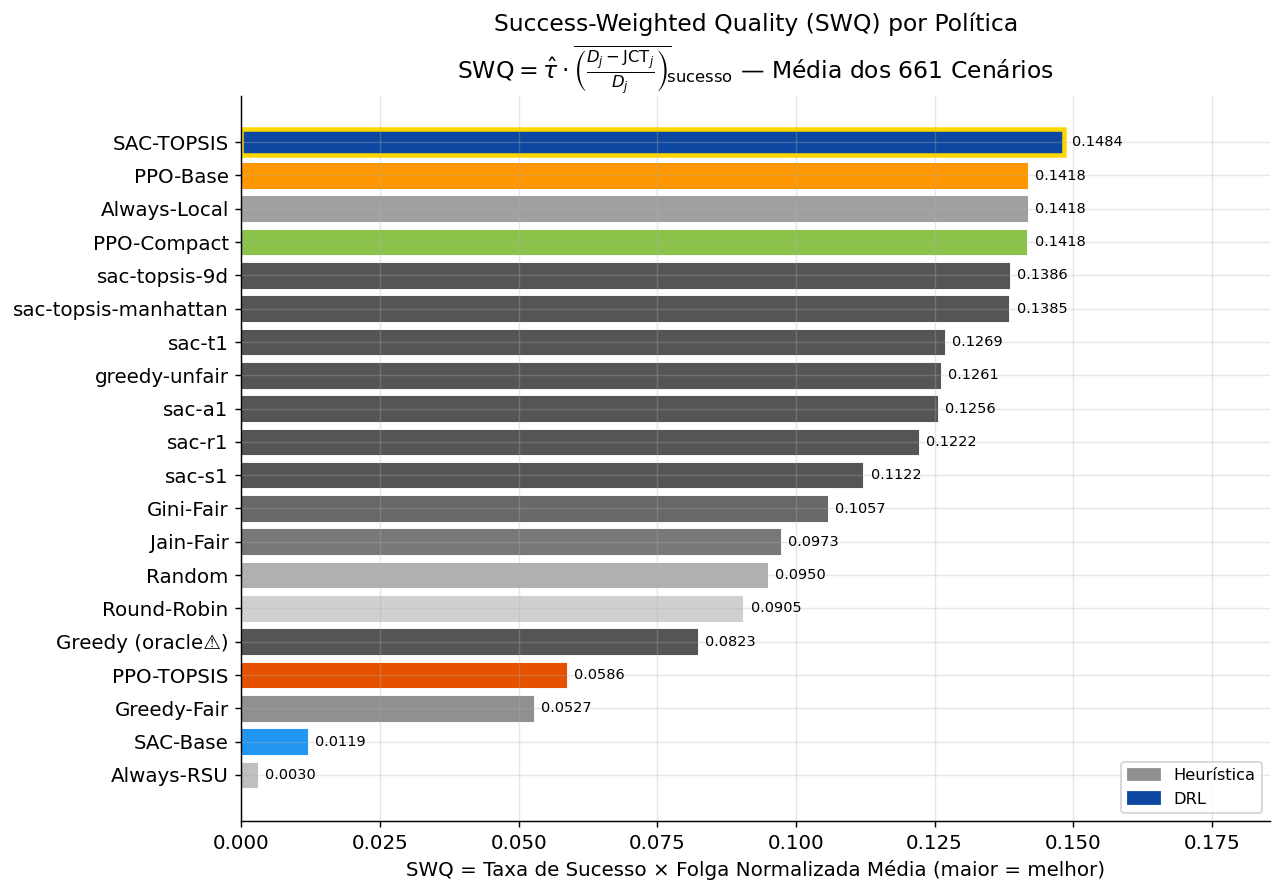
\includegraphics[width=\textwidth]{figuras/performance_09_swq.png}
\caption{SWQ médio por política sobre 661 cenários de teste ($\alpha=0{,}35$, $\beta=0{,}35$, $\gamma=0{,}30$). Barras em cinza representam heurísticas; barras escuras representam políticas \gls{DRL}. A borda dourada indica a melhor política. Maior é melhor.}
\label{fig:swq}
\end{figure}

\section{Por que o \gls{TOPSIS} agrega valor ao \gls{SAC} mas não ao \gls{PPO}?}
\label{sec:sac-topsis-sinergia}

Os resultados experimentais revelam uma assimetria marcante: o \gls{TOPSIS} eleva a taxa de \textit{deadline} do \gls{SAC} de $4{,}6\%$ (SAC-Base) para $45{,}3\%$ (SAC-TOPSIS), um ganho de $+40{,}7$ pontos percentuais, enquanto o \gls{PPO} com \gls{TOPSIS} regride. Para isolar a causa desta assimetria, foram realizados dois experimentos controlados. Primeiro, o PPO-TOPSIS original com estado 12D e ação ternária --- que permitia ao agente escolher entre rank$_1$, rank$_2$ e rank$_3$ --- obteve $18{,}4\%$, abaixo do PPO-Base ($42{,}4\%$). Segundo, o PPO-TOPSIS foi refatorado para utilizar \emph{exatamente} o mesmo estado 6D, ação binária $\{0\!=\!\text{LOCAL},\, 1\!=\!\text{rank}_1\}$ e função de recompensa do SAC-TOPSIS, diferindo apenas no algoritmo de otimização (\gls{PPO} vs.\ \gls{SAC}). O resultado deste experimento controlado foi igualmente $18{,}4\%$, com a política colapsando para $86\%$ de \textit{offload} via rank$_1$ --- o oposto do PPO-Compact ($100\%$ LOCAL), porém igualmente disfuncional. O PPO-TOPSIS-Compact, que usa o estado 6D mas foi treinado em cenários distintos, apenas iguala o PPO-Base. Em síntese: \textbf{o \gls{TOPSIS} é uma alavanca decisiva para o \gls{SAC} e um fator neutro ou prejudicial para o \gls{PPO}, independentemente do design do estado}. Esta seção analisa as causas estruturais desta assimetria.

\subsection{O problema do aprendizado redundante no PPO-TOPSIS}

O PPO-TOPSIS foi implementado com um estado de 12 dimensões --- três alternativas (LOCAL, \gls{RSU}, \gls{V2V}) ordenadas pelo escore \gls{TOPSIS}, cada uma descrita por quatro atributos normalizados (JCT estimado, energia, distância, \textit{link lifetime}) --- e um espaço de ação ternário $a_t \in \{0\!=\!\text{rank}_1,\, 1\!=\!\text{rank}_2,\, 2\!=\!\text{rank}_3\}$. Esse design cria um problema de \textbf{aprendizado redundante}: o \gls{TOPSIS} já determina deterministicamente que o candidato na posição 0 é o melhor segundo critérios multicritério rigorosos. O agente \gls{PPO}, portanto, é treinado por reforço para redescobrir, por tentativa e erro, o que o \gls{TOPSIS} já computou de forma ótima. A informação de valor genuíno que o agente deveria aprender --- se há benefício em descarregar para o melhor candidato dado o estado da fila e a urgência do \textit{deadline} --- está enterrada sob o sinal dominante de que rank$_1$ é sempre superior a rank$_2$ e rank$_3$ em custo multicritério.

O SAC-TOPSIS resolve este problema por projeto: delega a pergunta \emph{``para onde descarregar?''} inteiramente ao \gls{TOPSIS} e reserva ao agente apenas a pergunta \emph{``descarregar ou não?''} --- uma decisão genuinamente nova, que o \gls{TOPSIS} não responde, pois envolve a comparação entre o melhor candidato de \textit{offload} e a execução local ponderada pela urgência temporal, pelo congestionamento da fila e pela vantagem objetiva $\Delta_{\text{obj}}$ codificada no estado 6D.

\subsection{Colapso de política induzido pelo sinal TOPSIS}

O segundo mecanismo de falha do PPO-TOPSIS é o \textbf{colapso de política}. Com o estado 12D, a posição rank$_1$ exibe consistentemente JCT menor, energia menor e distância menor que rank$_2$ e rank$_3$. Isso gera um gradiente de política fortemente unidirecional desde as primeiras iterações: $P(a\!=\!0) \to 1$. O \gls{PPO} utiliza coeficiente de entropia $\alpha_{\text{ent}} = 0{,}01$, dez vezes menor que o do \gls{SAC} ($\alpha_{\text{ent}} = 0{,}10$ com ajuste automático via gradiente dual). Com entropia tão fraca, uma vez que a distribuição de política colapsa para $P(\text{rank}_1) \approx 1$, as trajetórias coletadas nas iterações seguintes são quase exclusivamente de escolhas rank$_1$, reforçando o colapso. O mecanismo de \textit{clipping} do \gls{PPO} ($\epsilon = 0{,}2$) não reverte esse estado: ele apenas impede mudanças \emph{grandes} por passo, mas não impede a deriva acumulada durante os 400 episódios de treinamento.

O \gls{SAC}, ao contrário, opera sobre um espaço de ação binário em que nenhuma das duas opções (LOCAL ou \textit{offload} para rank$_1$) domina o outro de forma incondicional: há cenários em que a fila do \gls{RSU} está saturada, ou o \gls{V2V} está distante, ou o \textit{deadline} é tão apertado que mesmo o melhor candidato de \textit{offload} não chega a tempo. Nesses casos, a resposta correta é LOCAL, e o sinal de recompensa deadline-aware --- com lacuna mínima de $1{,}5$ entre o melhor valor de falha e o pior valor de sucesso --- preserva um gradiente exploratório relevante. A alta temperatura entrópica do \gls{SAC} garante que ambas as ações recebam probabilidade não nula ao longo do treinamento, evitando o colapso.

\subsection{Assimetria de eficiência amostral com cenário único}

O protocolo de treinamento emprega \textbf{um único cenário} (\texttt{cenario\_v2x\_10tps\_w01}) durante os 400 episódios, com generalização \textit{zero-shot} para os 661 cenários de teste. Essa escolha é compatível com o \gls{SAC}, mas estruturalmente adversa ao \gls{PPO}.

O \gls{SAC} mantém um \textit{replay buffer} de 50.000 transições e realiza atualizações com \textit{minibatch} de 1024 amostras por passo. Com aproximadamente 100 tarefas por episódio, as 40.000 transições coletadas ao longo dos 400 episódios são amostradas em média $\approx\!40$ vezes cada durante o treinamento --- uma reciclagem intensiva que extrai máxima informação de um conjunto de dados limitado. Além disso, a mistura de experiências de diferentes pontos do treinamento (política mais aleatória nos primeiros episódios, mais refinada nos últimos) cria uma diversidade implícita que previne o sobreajuste ao único cenário de treino.

O \gls{PPO}, sendo \textit{on-policy}, descarta cada lote de trajetórias após as $k\!=\!8$ épocas de atualização. Com um único cenário, cada episódio gera essencialmente o mesmo padrão de chegada de tarefas, o mesmo volume de tarefas e as mesmas condições de canal. A política converge rapidamente para a estratégia que maximiza a recompensa nesse cenário específico --- que, com a salência do sinal \gls{TOPSIS}, é \emph{``sempre escolha rank$_1$''} --- e não tem como escapar desse ótimo local por falta de diversidade nos dados on-policy.

A evidência experimental confirma esta hipótese: o PPO-TOPSIS-Compact, que usa o estado 6D do SAC-TOPSIS (idêntico em conteúdo semântico) mas com algoritmo \gls{PPO}, atinge $42{,}4\%$ --- o mesmo que o PPO-Base, que usa o estado bruto 11D. O estado \gls{TOPSIS} mais informativo não agrega valor ao \gls{PPO} porque o gargalo não é a qualidade do estado, mas a ineficiência amostral do algoritmo on-policy com cenário único.

\subsection{Síntese: complementaridade estrutural SAC--TOPSIS}

A superioridade do SAC-TOPSIS não decorre de nenhum componente isolado, mas da \textbf{complementaridade estrutural} entre os dois módulos em três dimensões:

\begin{enumerate}
    \item \textbf{Divisão de responsabilidades}: O \gls{TOPSIS} resolve deterministicamente a pergunta \emph{``qual candidato de \textit{offload} é melhor?''}; o \gls{SAC} aprende a resposta à pergunta complementar \emph{``vale a pena descarregar para esse candidato?''}. As duas perguntas são independentes e igualmente necessárias; nenhum dos dois módulos, isoladamente, as responde ambas.

    \item \textbf{Off-policy + replay buffer}: O \gls{SAC} recicla cada transição $\approx\!40$ vezes no treinamento com um único cenário, alcançando uma eficiência amostral inacessível ao \gls{PPO} on-policy. Essa reciclagem é segura porque o \gls{SAC} aprende uma função de valor $Q(s,a)$ que é off-policy por construção --- ao contrário do \gls{PPO}, cujo gradiente de política requer dados coletados pela política corrente.

    \item \textbf{Regularização entrópica intensa}: O \gls{SAC} mantém $\alpha_{\text{ent}} = 0{,}10$ com ajuste automático, dez vezes superior ao coeficiente fixo do \gls{PPO}. Essa entropia elevada é precisamente o que impede o colapso de política frente ao sinal claro fornecido por $\Delta_{\text{obj}}$ no estado 6D --- mantendo a exploração ativa mesmo quando o \gls{TOPSIS} sugere fortemente que \textit{offload} é melhor.
\end{enumerate}

Em contraste, o PPO-TOPSIS sofre das três falhas simétricas: aprende uma pergunta que o \gls{TOPSIS} já responde (redundância), colapsa para uma estratégia degenerada com entropia insuficiente para resistir ao sinal \gls{TOPSIS} (colapso), e sobreajusta ao único cenário de treino sem o mecanismo de reciclagem do \textit{replay buffer} (ineficiência amostral). O experimento controlado confirma inequivocamente este diagnóstico: ao trocar \emph{apenas} o algoritmo --- mantendo estado 6D, ação binária e recompensa idênticos --- o SAC-TOPSIS atinge $45{,}3\%$ enquanto o PPO-TOPSIS obtém $18{,}4\%$, um déficit de $26{,}9$ pontos percentuais atribuível exclusivamente à natureza on-policy do \gls{PPO} e à sua baixa temperatura entrópica. O \gls{TOPSIS}, portanto, não é neutro quando mal integrado: \emph{amplifica} as fraquezas do algoritmo hospedeiro.

% ──────────────────────────────────────────────────────────────────────────────
\section{Avaliação Comparativa de Políticas}
\label{sec:ranking-completo}

As Tabelas~\ref{tab:ranking-completo} e~\ref{tab:ganho-topsis} resumem os resultados de 25 políticas avaliadas em 658 cenários de teste comuns, abrangendo algoritmos de aprendizado por reforço (com e sem \gls{TOPSIS}) e heurísticas de referência. As métricas reportadas são: taxa de \textit{deadline} (\%), SWQ ($= \hat{\tau}\cdot\overline{(D_j - \text{JCT}_j)/D_j}_{\text{sucesso}}$), JCT médio em segundos, energia média por tarefa em joules e o objetivo $J(\pi) = 0{,}60\cdot\hat{\tau} - 0{,}40\cdot\overline{(0{,}35\,\text{JCT} + 0{,}35\,E)/(D + 0{,}35\,E_{\max})}$ com $E_{\max} = 432{,}6\,\text{J}$ (percentil 99 global).

\begin{landscape}
\begin{table}[htbp]
\centering
\caption{Ranking completo das 25 políticas avaliadas em 658 cenários comuns (ordenado por SWQ decrescente). $\star$~=~usa \gls{TOPSIS}.}
\label{tab:ranking-completo}
\resizebox{\linewidth}{!}{%
\begin{tabular}{clrrrrrrrrr}
\toprule
\textbf{\#} & \textbf{Política} & \textbf{Cn} & \textbf{Taxa\%} & \textbf{SWQ} & \textbf{JCT (s)} & \textbf{E (J)} & \textbf{J($\pi$)} & \textbf{\%Loc} & \textbf{\%V2V} & \textbf{Categoria} \\
\midrule
 1 & \textbf{sac-topsis} $\star$       & 658 & \textbf{45,21} & \textbf{0,1484} &  6,547 & 25,828 & \textbf{0,2454} & 74,1 & 25,9 & RL+TOPSIS \\
 2 & ppo-topsis $\star$                & 658 & 42,66 & 0,1426 &  5,895 & 21,333 & 0,2344 & 98,7 &  1,3 & RL+TOPSIS \\
 3 & ppo-base                    & 658 & 42,32 & 0,1418 &  6,045 & 24,414 & 0,2295 & 100,0 &  0,0 & RL-Base \\
 4 & ppo-topsis-compact $\star$        & 658 & 42,32 & 0,1418 &  6,045 & 24,414 & 0,2295 & 100,0 &  0,0 & RL+TOPSIS \\
 5 & td3-base                    & 658 & 42,32 & 0,1418 &  6,045 & 24,414 & 0,2295 & 100,0 &  0,0 & RL-Base \\
 6 & a2c-topsis $\star$                & 658 & 42,32 & 0,1418 &  6,045 & 24,414 & 0,2295 & 100,0 &  0,0 & RL+TOPSIS \\
 7 & td3-topsis $\star$                & 658 & 43,91 & 0,1388 &  \textbf{3,703} & 22,995 & 0,2424 & 76,5 & 23,5 & RL+TOPSIS \\
 8 & sac-topsis-9d $\star$             & 658 & 42,82 & 0,1386 &  5,886 & \textbf{20,985} & 0,2348 & 94,7 &  5,3 & RL+TOPSIS \\
 9 & sac-topsis-manhattan $\star$      & 658 & 41,66 & 0,1385 & 11,831 & 23,656 & 0,2211 & 51,1 & 48,9 & RL+TOPSIS \\
10 & sac-t1 $\star$                    & 658 & 32,96 & 0,1270 & 11,487 & 26,126 & 0,1658 & 22,6 & 77,4 & RL+TOPSIS \\
11 & greedy-unfair               & 658 & 41,29 & 0,1262 &  5,613 &  7,396 & 0,2370 & 67,3 & 32,7 & Heurística \\
12 & sac-a1                      & 658 & 39,11 & 0,1256 & 13,722 & 21,118 & 0,2064 & 82,9 & 17,1 & RL-Base \\
13 & sac-r1                      & 658 & 38,26 & 0,1223 & 13,353 & 31,425 & 0,1914 & 58,8 & 41,2 & RL-Base \\
14 & sac-s1                      & 658 & 28,69 & 0,1122 & 39,298 & 20,305 & 0,1210 & 38,2 & 61,8 & RL-Base \\
15 & gini                        & 658 & 35,24 & 0,1057 &  3,456 & 39,395 & 0,1790 & 61,7 & 38,3 & Heurística \\
16 & dqn-topsis $\star$                & 658 & 25,90 & 0,0997 & 21,722 & 23,979 & 0,1161 & 20,0 & 80,0 & RL+TOPSIS \\
17 & jain                        & 658 & 32,54 & 0,0973 &  3,628 & 39,280 & 0,1627 & 58,6 & 41,4 & Heurística \\
18 & random                      & 658 & 30,02 & 0,0950 & 17,853 & 27,330 & 0,1427 & 40,7 & 59,3 & Heurística \\
19 & roundrobin                  & 658 & 28,50 & 0,0905 & 17,900 & 31,080 & 0,1315 & 34,9 & 65,1 & Heurística \\
20 & greedy                      & 658 & 29,03 & 0,0823 & 29,265 &  6,168 & 0,1429 & 42,5 & 57,5 & Heurística \\
21 & a2c-base                    & 658 & 21,74 & 0,0772 & 13,653 & 48,862 & 0,0785 & 20,3 & 79,7 & RL-Base \\
22 & dqn-base                    & 658 & 22,10 & 0,0686 & 13,599 & 44,445 & 0,0839 & 21,5 & 78,5 & RL-Base \\
23 & greedy-fair                 & 658 & 20,61 & 0,0528 & 40,754 &  \textbf{5,634} & 0,0823 & 27,9 & 72,1 & Heurística \\
24 & sac-base                    & 658 &  4,52 & 0,0119 & 57,075 & 24,230 & $-$0,042 &  5,1 & 94,9 & RL-Base \\
25 & rsu                         & 658 &  1,86 & 0,0030 & 144,191 & 4,843 & $-$0,123 &  1,2 & 98,8 & Heurística \\
\bottomrule
\end{tabular}%
}
\end{table}
\end{landscape}

A Tabela~\ref{tab:ganho-topsis} isola o efeito do \gls{TOPSIS} para cada família de algoritmos, comparando a versão base com a versão aumentada pelo ranqueamento multicritério.

\begin{table}[htbp]
\centering
\caption{Ganho do \gls{TOPSIS} por família de algoritmo (médias sobre 658 cenários comuns). $\Delta$Taxa e $\Delta$SWQ representam diferença absoluta; $\Delta$J($\pi$) é a diferença na função objetivo.}
\label{tab:ganho-topsis}
\small
\resizebox{\textwidth}{!}{%
\begin{tabular}{llrrrrrrr}
\toprule
\multirow{2}{*}{\textbf{Algoritmo}} & \multirow{2}{*}{\textbf{Versão}} & \multicolumn{2}{c}{\textbf{Taxa\%}} & \multicolumn{2}{c}{\textbf{SWQ}} & \multicolumn{2}{c}{\textbf{J($\pi$)}} & \multirow{2}{*}{\textbf{Destaques}} \\
\cmidrule(lr){3-4}\cmidrule(lr){5-6}\cmidrule(lr){7-8}
 & & Base & \gls{TOPSIS} & Base & \gls{TOPSIS} & Base & \gls{TOPSIS} & \\
\midrule
\multirow{2}{*}{SAC}
 & base   & 4,52  & ---    & 0,0119 & ---    & $-$0,042 & --- & colapso total (94,9\% \gls{V2V}) \\
 & topsis & ---   & \textbf{45,21} & ---    & \textbf{0,1484} & --- & \textbf{0,2454} & \textbf{$+$40,7 pp / $+$1147\% SWQ} \\
\midrule
\multirow{2}{*}{PPO}
 & base   & 42,32 & ---    & 0,1418 & ---    & 0,2295 & --- & 100\% local \\
 & topsis & ---   & 42,66  & ---    & 0,1426 & --- & 0,2344 & $+$0,3 pp / $+$0,6\% SWQ \\
\midrule
\multirow{2}{*}{TD3}
 & base   & 42,32 & ---    & 0,1418 & ---    & 0,2295 & --- & 100\% local \\
 & topsis & ---   & 43,91  & ---    & 0,1388 & --- & 0,2424 & $+$1,6 pp taxa; JCT $-44{,}5\%$ \\
\midrule
\multirow{2}{*}{DQN}
 & base   & 22,10 & ---    & 0,0686 & ---    & 0,0839 & --- & 78,5\% \gls{V2V} sem critério \\
 & topsis & ---   & 25,90  & ---    & 0,0997 & --- & 0,1161 & $+$3,8 pp / $+$45\% SWQ \\
\midrule
\multirow{2}{*}{A2C}
 & base   & 21,74 & ---    & 0,0772 & ---    & 0,0785 & --- & 79,7\% \gls{V2V}, energia alta \\
 & topsis & ---   & 42,32  & ---    & 0,1418 & --- & 0,2295 & \textbf{$+$20,6 pp / $+$84\% SWQ} \\
\bottomrule
\end{tabular}%
}
\end{table}
